\chapter{Conclusion}
\begin{quotation}\textit{
Man's last mind paused before fusion, looking over a space that included nothing but the dregs of one last dark star and nothing besides but incredibly thin matter, agitated randomly by the tag ends of heat wearing out, asymptotically, to the absolute zero.\\
Man said, ``AC, is this the end? Can this chaos not be reversed into the Universe once more? Can that not be done?''\\
AC said, ``THERE IS AS YET INSUFFICIENT DATA FOR A MEANINGFUL ANSWER.''
}
\begin{flushright}Isaac Asimov (The Last Question, 1956)\end{flushright}\end{quotation}

\lettrine{I}{ntro}
\chaptertoc

\section{Perspectives}
\label{chapter:perspectives}
\subsection{Micro}

Reinforcement learning, \citep{Marthi05concurrenthierarchical}


Evolving control policies, \citep{Miles2007}
\subsection{Tactics}

Two important research directions for tactics would be:
\begin{itemize}
    \item Tactical assault generation, so that we do not have to hard-code the tactical goals behaviors. Previous works, which would be compatible with StarCraft, in this direction include \citep{Chung05,PonsenMSA06,UCT}.
    \item Improve tactical state estimation, so that both our tactical decision-making and tactical prediction benefit it. A first step would be to use a (dynamic) filtering on enemy units, either with a particle filter \citep{Thrun02d,weber2011aiide} or with hidden semi-Markov models \citep{Hladky_anevaluation}. We propose here a simple units filtering model based on the decomposition of the map in regions.
\end{itemize}

\subsubsection{Enemy Units Filtering}
We consider a simple model, without speed nor steering nor $See$ variable for each position/unit. The fact that we see positions where the enemy units are is taken into account during the update.
The idea is to have (learn) a multiple influences transition matrix on a Markov chain on top the regions discretization (see chapter~\ref{chapter:tactics}), which can be seen as one Markov chain for each combination of motion-influencing factors.

The \textbf{perception} of such a model would be for each unit if it is in a given region, as the bottom diagram in Figure~\ref{fig:BWTA}. From there, we can consider either map-dependent regions, regions uniquely identified as they are in given maps that is; or we can consider regions labeled by their utility. We prefer (and will explain) this second approach as it allows our model to be applied on unknown (never seen) maps directly and allows us to incorporate more training data. The regions get a number in the order in which they appear after the main base of the player (e.g. see region numbering in Fig.~\ref{fig:terrainanalysis} and~\ref{fig:examplefilter}). %For instance regions ordering is $1 \rightarrow main\_base, 2 \rightarrow first\_expansion, 3 \rightarrow

\vspace{0.3cm}
\textit{Variables}\\
\vspace{0.5cm}
%There are $p$ regions, the full filter works on $m$ units, each of the units is represented by $n$ particles.
The full filter works on $n$ units, each of the units having a mass in the each of the $m$ regions.

%%% \begin{itemize}
%%%     \item $Agg \in \{T,F\}$, the player's aggressiveness (is he attacking or defending?), which can comes from other models but can also be an output here. 
%%%     \item $UT_{i \in \llbracket 1\dots m \rrbracket} \in \{unit\ types\}$ the type of the $i$th tracked unit.
%%%     \item $X^{t-1}_{i \in \llbracket 1\dots m \rrbracket , j \in \llbracket 1\dots n \rrbracket} \in \{regions\}\ i.e.\ \in \llbracket 1 \dots p \rrbracket$ the $j$th particle for the $i$th unit at time $t-1$.
%%%     \item $X^{t}_{i \in \llbracket 1\dots m \rrbracket , j \in \llbracket 1\dots n \rrbracket} \in \{regions\}$, the $j$th particle for the $i$th unit at time $t$.
%%% \end{itemize}
\begin{itemize}
    \item $Agg \in \{true,false\}$, the player's aggressiveness (is he attacking or defending?), which can comes from other models but can also be an output here. 
    \item $UT_{i \in \llbracket 1\dots n \rrbracket} \in \{unit\ types\}$ the type of the $i$th tracked unit.
    \item $X^{t-1}_{i \in \llbracket 1\dots n \rrbracket} \in \llbracket r_1 \dots r_p \rrbracket$, the $i$th unit at time $t-1$.
    \item $X^{t}_{i \in \llbracket 1\dots n \rrbracket} \in \llbracket r_1 \dots r_p \rrbracket$, the $i$th unit at time $t$.
\end{itemize}

%we have And the $Map \in \{maps\}$ variable for map dependent models. 

\vspace{0.3cm}
\textit{Joint Distribution}\\
\vspace{0.5cm}
We consider all units conditionally independent give learned parameters. (This may be too strong an assumption.) %(false, we could cluster armies: but we can hope the parameters will account for units traditionally moving together).\\

%%% \begin{eqnarray}
%%% & & \PP(Agg, UT_{1:m}, X^{t-1,t}_{1:m,1:n}) \\
%%% & = & \PP(Agg)\prod_{i=1}{m} \PP(UT_{i}\\
%%% & \times & \prod_{j=1}{n} \PP(X^{t-1}_{i,j} \PP(X^t_{i,j}|X^{t-1}_{i,1:n},UT_i,Agg)
%%% \end{eqnarray}
\begin{eqnarray}
& & \PP(Agg, UT_{1:m}, X^{t-1,t}_{1:m,1:n}) \\
& = & \PP(Agg)\prod_{i=1}^{n} \left[ \PP(UT_{i}) \PP(X^{t-1}_{i}) \PP(X^t_{i}|X^{t-1}_{i},UT_i,Agg)\right]
\end{eqnarray}

\vspace{0.3cm}
\textit{Forms}\\
\vspace{0.5cm}

\begin{itemize}
    \item $\PP(Agg)$ is a binomial distribution.
    \item $\PP(UT_i)$ is categorical distribution (on unit types).
    \item $\PP(X^{t-1}_{i}$ is a categorical distribution (on regions).
    \item $\PP(X^t_i|X^{t-1}_i,UT_i,Agg)$ are $\#\{units\_types\} \times \abs{Agg}$ different $m\times m$ matrices of transitions from regions to other regions depending on the type of unit $i$ and of the aggressiveness of the player. (We just have $\#\{units\_types\} \times \abs{Agg} \approx 15\times 2$ different matrices for each race.)
\end{itemize}


\vspace{0.3cm}
\textit{Identification (learning)}\\
\vspace{0.5cm}

$\PP(X^t_i|X^{t-1}_i, UT_i, Agg)$ is learned with a Laplace rule of succession from previous games. Against a given player and/or on a given map, one can use $\PP(X^t_i|X^{t-1}_i, UT_i, Agg, Player, Map)$ and use the learned transitions matrices as priors. When a player attacks in the dataset, we can infer she was aggressive at the beginning of the movements of the army which attacked. When a player gets attacked, we can infer she was defensive at the beginning of the movements of the army which defended. At other times, $\PP(Agg=true) = \PP(Agg=false) = 0.5$.
\begin{eqnarray*}
& & PP(X^t_i=r|X^{t-1}_i=r', UT_i=ut, Agg=agg) \\
& \propto & \frac{1+n_{transitions}(r'\rightarrow r, ut, agg)\PP(agg)}{\#\{entries\_to\_r\} + \sum_{j=1}^{m} n_{transitions}(r' \rightarrow r_j, ut, agg)\PP(agg)}
\end{eqnarray*}

\vspace{0.3cm}
\textit{Update (filtering)}\\
\vspace{0.5cm}

\begin{itemize}
    \item When a unit $i$ becomes hidden, which was seen in region $r$ just before, we have:
\begin{eqnarray*}
\begin{cases}
\PP(X^t_{i} = r) = 1.0\\
\PP(X^t_{i} = j) = 0.0\ \mathrm{iff}\ j \neq r
\end{cases}
\end{eqnarray*}

    \item For all regions $r$ that we see ``totally'' (above a threshold of a percentage of the total area), we set $\PP(X^t_i = r) = 0.0$ and redistribute their probability mass to hidden (or still partially hidden) regions (algorithm~\ref{alg:cullingfilter}):
\begin{algorithm}[!h]
\caption{Culling/updating algorithm for filtering visible regions}
\label{alg:cullingfilter}
\begin{algorithmic}
\ForAll{$i \in \{enemy\_units\}$}
    \State $s \leftarrow 0.0$
    \ForAll{$r \in \{visible\_regions\}$}
        \State $s \leftarrow s + \PP(X^{t-1}_i = r)$
        \State $\PP(X^{t-1}_i = r) = 0.0$
    \EndFor
    \State $total \leftarrow \sum_{j=1}^m \PP(X^{t-1}_i=r_j)$
    %\State $k \leftarrow \#\{\neg visible\_regions\}$
    \ForAll{$r \in \{\neg visible\_regions\}$}
        \State $\PP(X^t_i = r) \leftarrow \PP(X^t_i = r) + \frac{s}{total}\times \PP(X^{t-1}_i = r)$
    \EndFor
\EndFor
\end{algorithmic}
\end{algorithm}

    \item For all the other cases, we have:
$$\PP(X^t_{i} = r) = \sum_{j=1}{m} \PP(X^{t-1}_i = r')\PP(X^t_i = r | X^{t-1}_i = r', UT_i, Agg)$$
\end{itemize}

\vspace{0.3cm}
\textit{Questions}\\
\vspace{0.5cm}

\begin{itemize}
    \item When we want to infer where the $n$ enemy units are, we ask:
\begin{eqnarray*}
& & \PP(X_{1:n}^t| UT_{1:n}=ut_{1:n})\\
& \propto= & \sum_{Agg} \PP(Agg) \prod_{i=1}^n \PP(ut_i) \sum_{X_i^{t-1}} \PP(X_i^t|X_i^{t-1},ut_i,Agg)\\
& \propto & \sum_{agg=false}^{true} \PP(Agg) \prod_{i=1}^n \PP(UT_i=ut_i) \sum_{r = 1}^{m} \PP(X_i^t|X_i^{t-1}=r,ut_i,Agg=agg)
\end{eqnarray*}
    \item When we want to infer the aggressiveness of the enemy (from the troupes' movements that we have seen), we ask:
\begin{eqnarray*}
& & P(Agg | UT_{1:n} = ut_{1:n})\\
& \propto & \PP(Agg) \prod_{i=1}^{n} \PP(ut_i)\sum_{X_i^t}\PP(X_i^{t-1}) \sum_{X_i^{t-1}}  \PP(X_i^t|X_i^{t-1},ut_i,Agg) 
\end{eqnarray*}
\end{itemize}

\vspace{0.3cm}
\textit{Conclusion}\\
\vspace{0.3cm}

Offline learning of matrices (as shown in Fig.~\ref{fig:examplefilter}) of aggressive and defensive probable region transitions (for a given unit type). With online learning (taking previous offline learned parameters as priors), we could learn preferences of a given opponent.

\begin{figure}
\begin{center}
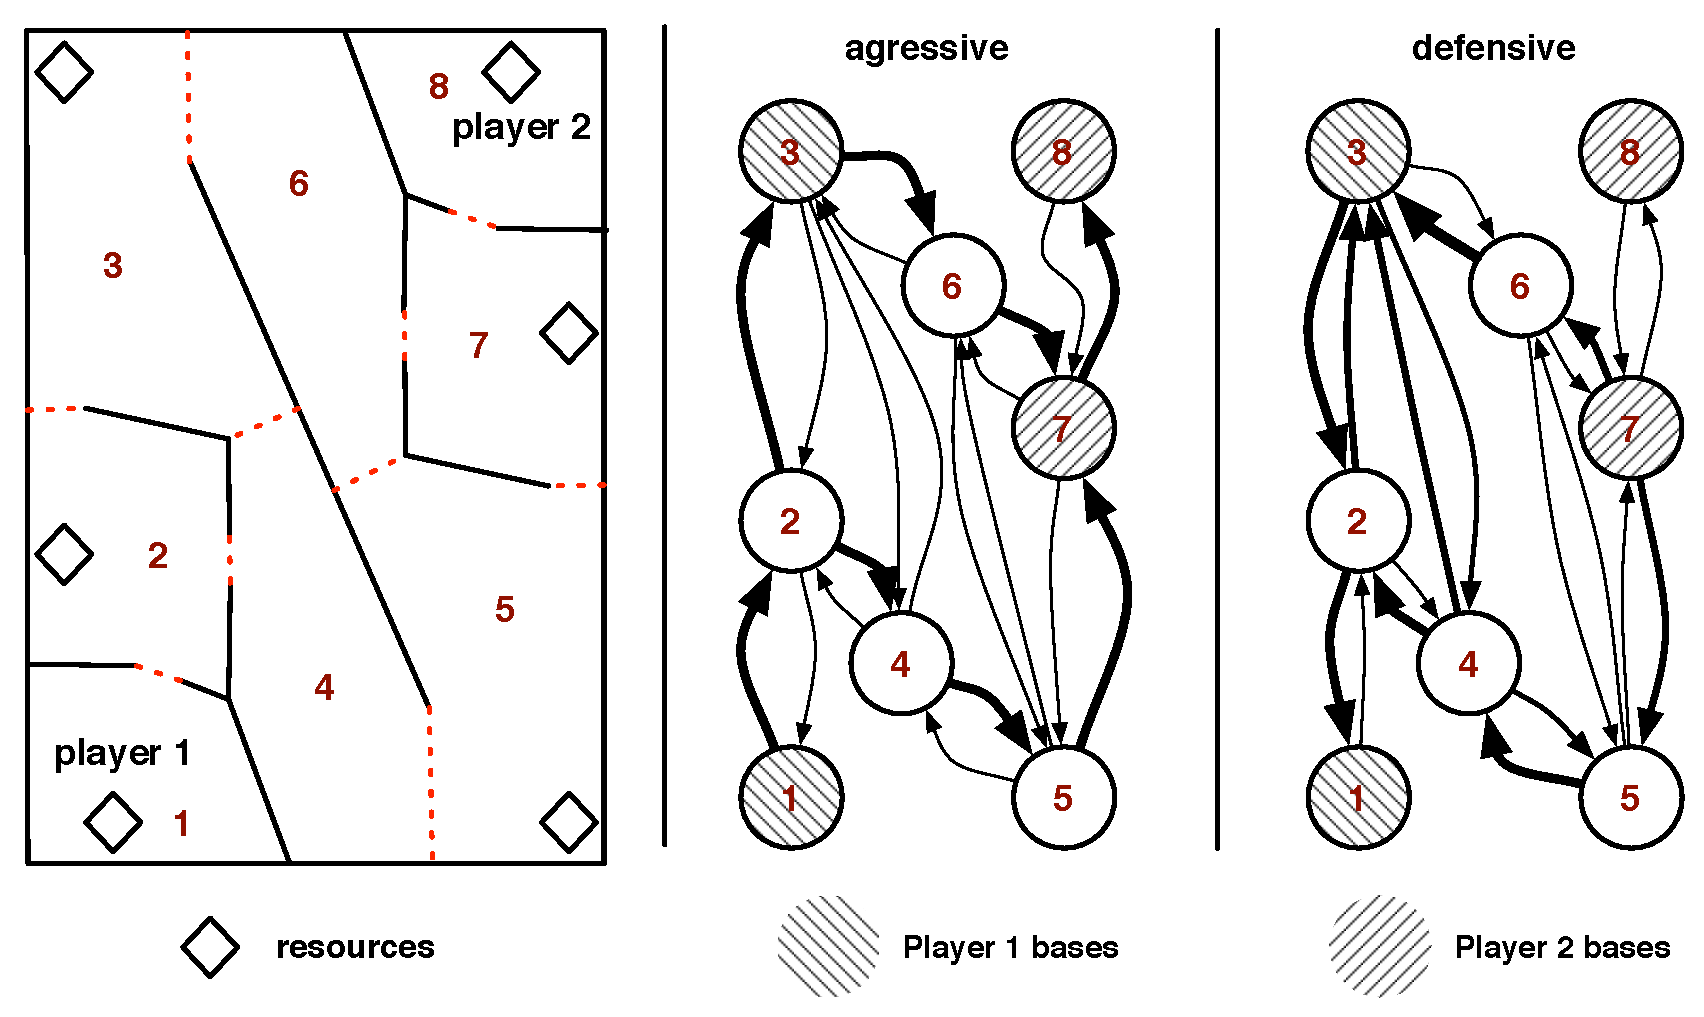
\includegraphics[width=15cm]{images/units_filter_markov.pdf}
\caption{Example of the units filter transition matrices on a simple map (same as in Fig.~\ref{fig:terrainanalysis}) for aggressive and defensive sets of parameters for a given unit type. The thickness of the arrows is proportional to the transition probability between regions.
\label{fig:examplefilter}
\end{center}
\end{figure}

By considering a particle filter, we could consider a finer model in which we deal with positions of units (in pixels or walk tiles or build tiles) directly, but there are some drawbacks:
\begin{itemize}
    \item The data to learn (offline or online) is sparse as there are several versions of the same map and the combinatorics of start positions (2 occupied start positions on 4 possible most of the time). This would need any form of spatial abstraction anyway, like distance to most walked traces.
    \item Computation cost to track $\approx 40$ units makes it so that the particle sampling numbers should be low to stay real-time. Or that one should abandon the motion model for a Kalman filter \citep{Kalman1960}. 
\end{itemize}
The advantages are not so strong: 
\begin{itemize}
    \item (hopefully) more precision in units position estimation,
    \item possibilities to have more complex motion models (updates/culling of the filter),
    \item differentiation between trajectories of ground and flying units,
    \item differentiation between different trajectories of attacks inside large regions.
\end{itemize}



\subsection{Strategy}
Bandits (contextual bands)\\
Planning \citep{Wolfe11}\\
Probabilistic planning?

\subsection{Inter-game Adaptation (Meta-game)}
Other cases of learning not dealt with in previous chapters:
\citep{metalevelbehavioradaptrts}
Laplace smoothing $P(ETT=ett|Player=p)= \frac{1 + nbgames(ett,p)}{\#ETT + nbgames(p)}$. Same for $EClusters$ and $ETactics$.\\

The full (reinforcement) learning of the bot can be seen as learning degrees of liberty one by one with a hierarchy from strategies to actions by tactics. C.f R-IAC Baranes \& Oudeyer 2009 and 2012; $PI^2$-CMA (ES).\\

meta question I think that he thinks that I think that...

\section{Contrib}
Résumer les contributions
\subsection{Approaches}
%%% \begin{itemize}
%%% \item train your IA from data
%%% \item or train your IA by itself
%%% \item or let the game designers set the parameters
%%% \end{itemize}
\begin{itemize}
\item A tractable decomposition of game AI in a hierarchy of predictions, decisions and actions.
\item Integration of learning in a decision-making model. 
\item An autonomous agent for StarCraft (BroodwarBotQ).
\end{itemize}

\subsection{Results}
Recall what works, what should be extended.

\section{Perspectives: Not a solved problem yet}
Computers don't beat good (experts) humans (higher level strategic thinking: common sense, plus vision/interpolation for efficient micro). They are not so fun (do not adapt that much, our bot is the most adaptive ATM). Competition results.
Tout ce qui peut se faire en recherche et ce qui est directement applicable par l'industrie.


